\documentclass{article}
\usepackage{amsmath} % Example package usage
\usepackage{graphicx} % For including images

\begin{document}

\title{Introduction to Neural Networks}
\author{Arnav Singhal}
\date{\today}
\maketitle

\begin{abstract}
This document provides an overview of neural networks, including their structure, mathematical representation, training process and common notations used in the field.
\end{abstract}

\tableofcontents

\section{Overview} \label{sec:overview}
Neural networks are computational models inspired by the human brain. They consist of interconnected nodes, or \textbf{neurons}, arranged in layers. The basic components of a neural network include:

\begin{itemize}
    \item Input Layer
    \item Hidden Layers
    \item Output Layer
\end{itemize}

\section{Mathematical Representation} \label{sec:math}
Mathematically, a neuron processes input $x_i$ with associated weights $w_i$ and a bias $b$:

\begin{equation} \label{eq:neuron}
    y = f\left( \sum_{i=1}^{n} w_i x_i + b \right)
\end{equation}

where $f$ is the activation function. Common choices for $f$ include:

\subsection{Activation Functions} \label{subsec:activation}
\begin{enumerate}
    \item Sigmoid: $f(x) = \frac{1}{1+e^{-x}}$
    \item ReLU: $f(x) = \max(0, x)$
    \item Tanh: $f(x) = \frac{e^x - e^{-x}}{e^x + e^{-x}}$
\end{enumerate}

\section{Training Process} \label{sec:training}
The learning process involves updating the weights using an optimization algorithm like \textit{gradient descent}. Given a loss function $L$, the weight update follows:

\begin{align} \label{eq:weight_update}
    w_{new} &= w_{old} - \eta \frac{\partial L}{\partial w} \\
    b_{new} &= b_{old} - \eta \frac{\partial L}{\partial b}
\end{align}

Equation \eqref{eq:neuron} describes the neuron function, and the weight update rule is shown in \eqref{eq:weight_update}.

\section{Greek Letters in Neural Networks} \label{sec:greek}
Neural networks often use Greek letters for notation:

\begin{itemize}
    \item $\alpha$ (learning rate)
    \item $\theta$ (model parameters)
    \item $\lambda$ (regularization parameter)
\end{itemize}

\section{Illustration} \label{sec:illustration}
An example of a neural network structure is shown below:

\begin{center}
    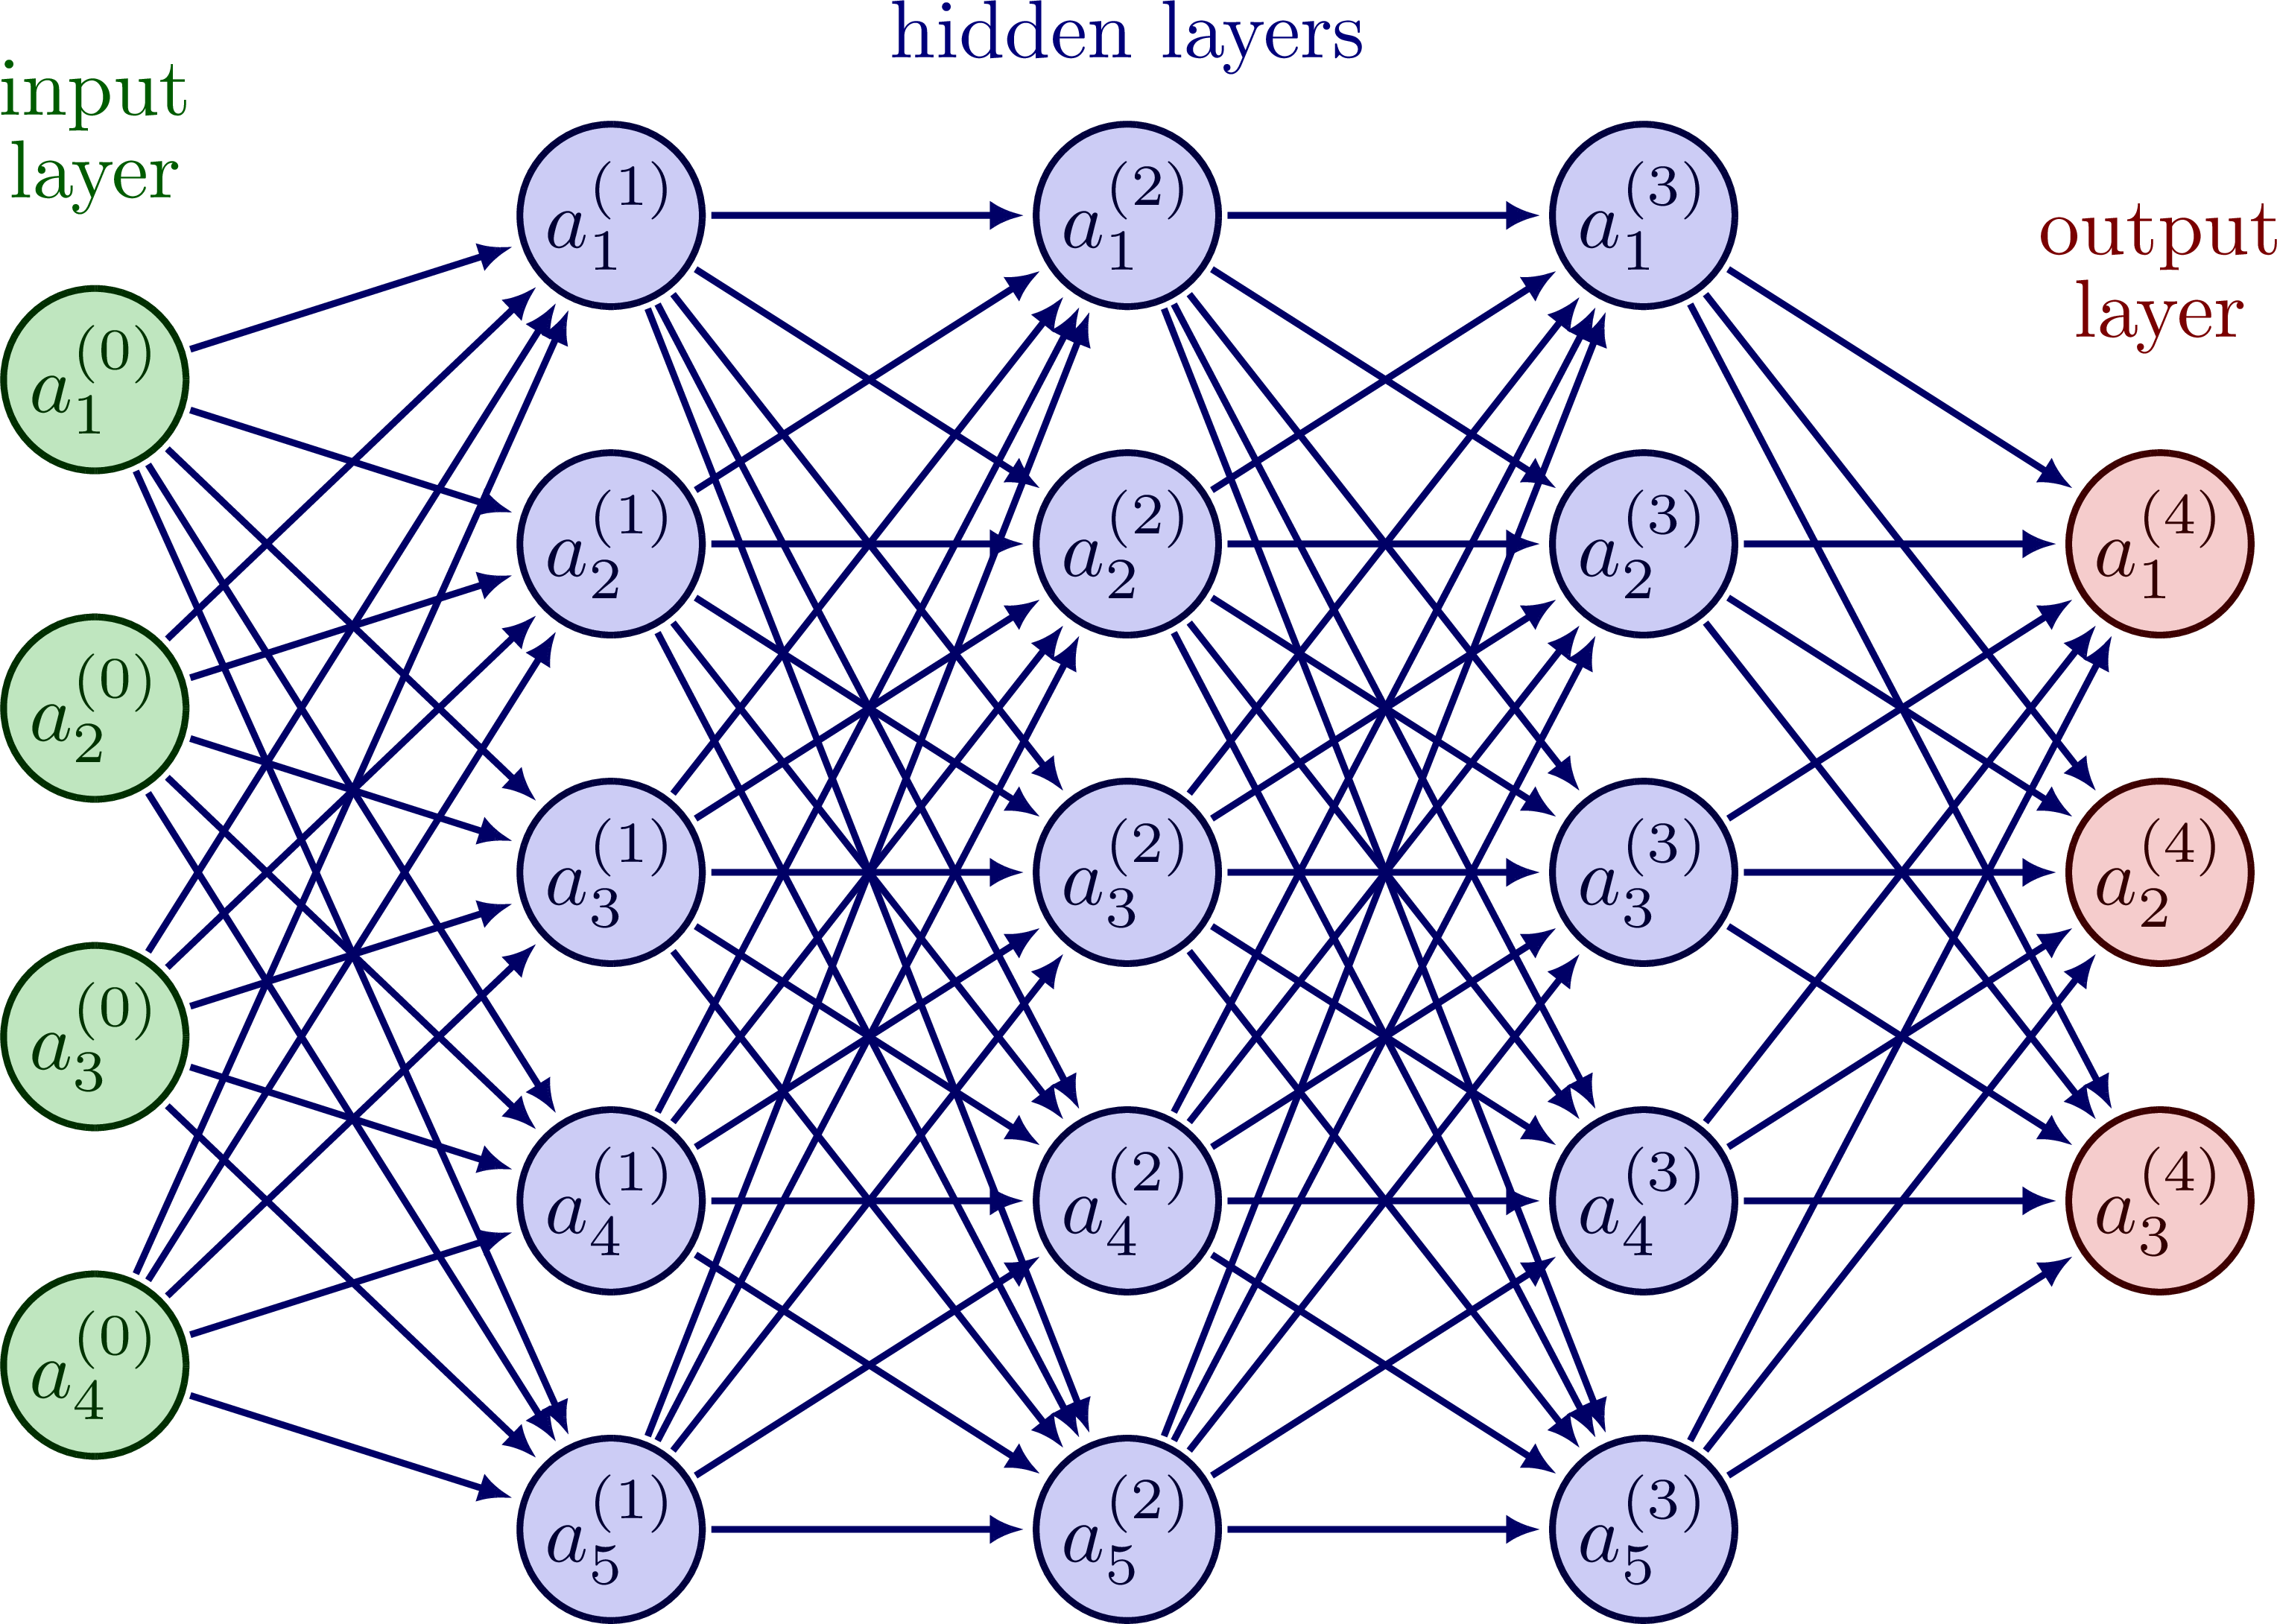
\includegraphics[width=0.5\textwidth]{neural_networks.png} % Example image
\end{center}

\section{Neural Network Parameters} \label{sec:parameters}
The following table summarizes key parameters of a neural network:

\begin{table}[h]
    \centering
    \begin{tabular}{|c|c|}
        \hline
        Parameter & Description \\
        \hline
        $w$ & Weights of connections \\
        $b$ & Bias term \\
        $\alpha$ & Learning rate \\
        $L$ & Loss function \\
        \hline
    \end{tabular}
    \caption{Neural Network Parameters}
    \label{tab:parameters}
\end{table}

\section{Conclusion} \label{sec:conclusion}
Neural networks are a powerful tool for pattern recognition and machine learning. Understanding their structure and training mechanisms is crucial for implementing AI systems.

\begin{thebibliography}{9}

\bibitem{ref1} Y. LeCun, Y. Bengio, and G. Hinton. "Deep learning." *Nature*, vol. 521, no. 7553, 2015, pp. 436-444.

\bibitem{ref2} I. Goodfellow, Y. Bengio, and A. Courville. *Deep Learning*. MIT Press, 2016.

\bibitem{ref3} D. P. Kingma and J. Ba. "Adam: A method for stochastic optimization." *International Conference on Learning Representations (ICLR)*, 2015.

\bibitem{ref4} X. Glorot and Y. Bengio. "Understanding the difficulty of training deep feedforward neural networks." *International Conference on Artificial Intelligence and Statistics (AISTATS)*, Sardinia, Italy, 2010.

\bibitem{ref5} A. Krizhevsky, I. Sutskever, and G. Hinton. "ImageNet classification with deep convolutional neural networks." *Advances in Neural Information Processing Systems (NeurIPS)*, 2012.

\end{thebibliography}

\end{document}